\chapter{Web-Based Responsive Spoken Dialogue System}
\label{chap:web-based_responsive_spoken_dialogue_system}

\lettrine{W}{ith} the ability to simulate accommodation, a complete accommodative \acl{sds} is introduced in this chapter.
Its architecture and various customization possibilities are explained.
The vocal changes are illustrated using dynamic visualizations in the system's \acl{gui}.
A replication of the \acl{hci} experiment is showcased to exhibit the system's capabilities and demonstrate its advantages.

\pagebreak

\acresetall

\section[Overview]{Overview and key aspects}
\label{sec:overview_and_key_aspects}

Simulating and triggering accommodation effects occurring in \ac{hhi} in \acp{sds} takes them one step further toward human-like communication.
The system presented in this chapter encapsulates the knowledge acquired from the experiments in \cref{part:experiments}, the behavior designs developed in \cref{part:modeling}, and the module introduced in \cref{chap:convergence_module_for_sdss}.
It contains mechanisms to track the states and changes of segment and suprasegmental phonetic features during a dialogue.
All analyses are automated and run in real-time, which not only saves a lot of time and manual work typically needed in accommodation studies, but also makes the system more suitable for use in other applications.
A user of the system may be a participant in an experiment, an experimenter designing an experiment or monitoring an ongoing experiment, or a researcher that uses it to analyze existing data.
The system was designed with the following key principles in mind:
%
\begin{description}
	\item[Focus on adaptation] --
	the main goal of the system is to offer a tool for investigating vocal accommodation in \ac{hci} for both online experiments and offline analyses.
	Putting vocal accommodation under the spotlight is the core novel contribution of the system, since very few systems offer such capabilities at all, and with control over the accommodative behavior in particular.
	
	\item[Customizability] --
	the system includes several components that can be modified, either for changing the accommodation behavior itself (features, parameters, etc.) or for changing the settings (e.g., for different experiments).
	This allows experimentation with customized scenarios and configurations that can be easily compared in a controlled, reproducible environment.
	
	\item[Online scalability] --
	the system can run in a web browser without any installations or additional files\footnote{Some features need to be enabled in the browser, like JavaScript and microphone access.
	However, any modern browser should not have any problem supporting all the necessary requirements.
	To increase performance, all speech analyses and processing are done on the server side.}.
	Since the system itself runs on a server, it is also possible to operate multiple instances, each with its own configurations and parameters.
	This makes it easy to distribute its use, e.g., for remotely conducting an experiment where a specific configurations can be given to each participant.
\end{description}
%
This customizable system is a tool that could help to deepen the experimental possibilities and to automate the processes typically involved in accommodation-related experiments.
The system's architecture, \ac{gui}, and functionality are described in \cref{sec:architecture,sec:online_and_offline_modes}.
The experiment presented in \cref{chap:shadowing_in_sung_music_and_human_computer_interaction} is replicated in \cref{sec:showcase} to demonstrate the system's utilization.

\section{Architecture}
\label{sec:architecture}

As the system aims to offer a customizable playground for studying phonetic adaptation in \ac{hci}, a key property of its architecture is the separation between client-side, server-side, and external resources (see \cref{fig:web-based_architecture}).
This separation makes it possible to run multiple clients on different machines at the same time with a single server collecting the data from all of them at the same time.
The server, ideally running on a dedicated machine, is operated by a person responsible for designing and configuring the interactions, e.g., an experimenter.
It collects information and audio recordings from all interactions with the system (which can be deleted afterwards for privacy purposes).
This separation of the server grants the experimenter a lot of freedom and flexibility, since resources like feature configurations and dialogue domain can be modified independently, even while users are using the system.
Additionally, multiple configurations can be prepared in advance (e.g., for different participant groups), regardless of the device the experiment will be performed on and without summoning the participants to the lab.
Configurations can even be changed over the course of the experiment if additional variations are required.
These configurations are transparent to the users, and no action is required from them aside from starting a new interaction with he system.
This flexibility makes it easier and quicker to create new scenarios of interaction and to experiment with different features and parameters.

In addition to the technical advantages, letting users to interact with the system on a separate machine broadens the usage possibilities.
For example, an experiment can be carried out remotely, without the need to invite participants to the recording studio one by one.
Furthermore, as the connection to the server is done via a web browser, participants can connect use the system with their own computers wherever and whenever it suits them, without any additional installation or technical configurations.
All of these make it possible to collect data from many users rapidly and easily.
%
\begin{figure}[t]
	\centering
	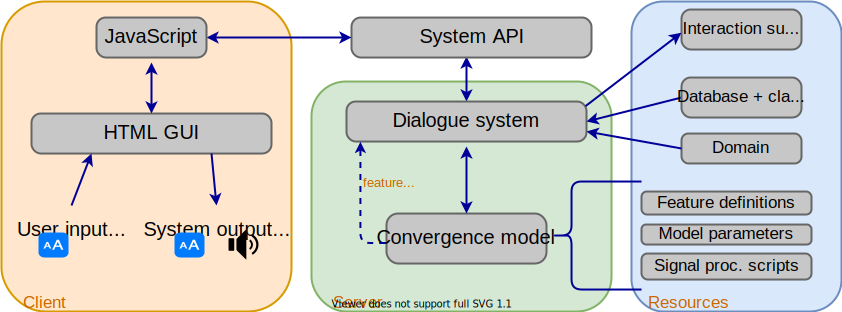
\includegraphics[width=\linewidth]{web-based_architecture_no-ajax}
	\caption[Architecture of the web-based system]
		{The architecture of the system.
		The background colors distinguish between client components, server components, and customizable external resources.
		The dashed line coming out of the convergence model's box indicates that the feature predictions may or may not be passed from the model to the system depending on the feature definition and update parameter (see \cref{sec:parameters}).}
	\label{fig:web-based_architecture}
\end{figure}
%
The main components of the system are the \ac{sds} with the accommodation module (\cref{subsec:dialogue_system}), the \ac{gui} (\cref{subsec:graphical_user_interface}), and the external resources and configuration (\cref{subsec:models_and_cusomizations}).

\subsection{Dialogue system}
\label{subsec:dialogue_system}

The core of the system is the dialogue system component (see green block in \cref{fig:web-based_architecture}), which controls the flow of the interaction, processes users' inputs, and generates the system's responses.
It uses the extended architecture presented in \cref{subsec:extended_sds}, which consists of traditional \ac{sds} components such as \ac{nlu} and a \ac{dm}, but also contains the \ac{asp} module that adds accommodation support \citep{Raveh2017SemDial}.
The implementation of this module in the system is as described in \cref{fig:adaptation_module_architecture}.
While the \ac{nlu} component uses merely the transcription provided by the \ac{asr}, the \ac{asp} module analyzes the speech signal itself.
Concretely, it tracks occurrences of the defined features and passes their measured values to the convergence model, as explained in \cref{subsubsec:tracked_features}, which, in turn, forwards the tracked feature parameters to the \ac{tts} synthesis component.
The \ac{tts} engine then takes the text generated by the \ac{nlg} component, and, if phonetic-level manipulation is supported by the \ac{tts} module, synthesizes the utterance using the values specified by the convergence model.
The connection between the dialogue system's modules is managed by the OpenDial framework \citep{Lison2016opendial, Lison2015developing}.
%The \ac{asr} module uses CMUSphinx \citep{Lamere2003sphinx} with additional customized functionality for obtaining the phonetic information required for the \ac{asp} module, and the \ac{tts} is driven by MaryTTS \citep{LeMaguer2017uprooted, Schroeder2003mary}.
The \ac{nlu} and \ac{nlg} modules are built using an OpenDial's domain file, as described in \cref{subsubsec:dialogue_domain}.
Importantly, each of these components can be replaced with another implementation, all time it takes the same input and provides the same type of output.

\subsection{Visualization and \acl{gui}}
\label{subsec:graphical_user_interface}

\afterpage{%
	\begin{landscape}
		\begin{figure}[t]
			\centering
			\vspace*{-2cm}
			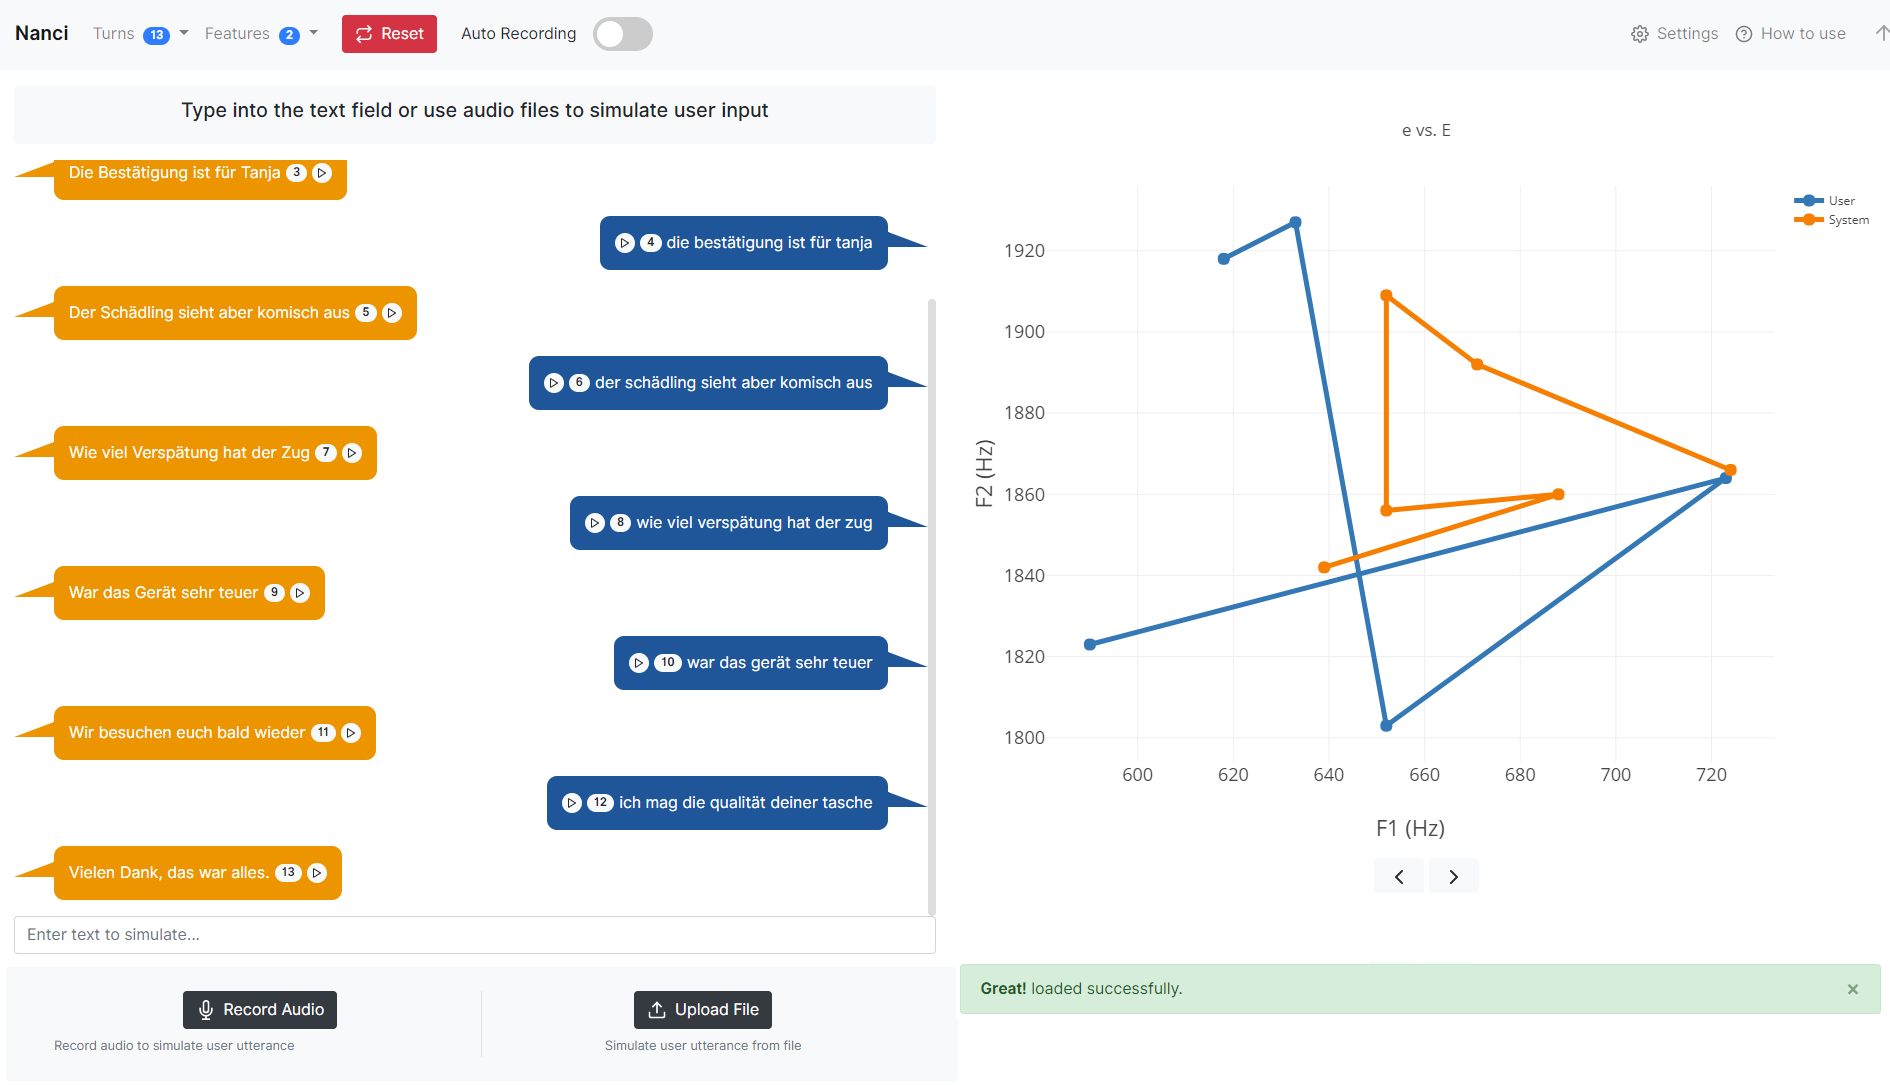
\includegraphics[width=\linewidth]{gui}
			\caption[Web system in-browser \acs{gui}]
				{A screenshot of the system's \acl{gui}, with the chat area on the top left, the interaction area on the bottom left, the plot area on the top right, and the notification area on the bottom right.
				In both the chat area and the plot area, the user and system are represented by the colors blue and orange, respectively.}
			\label{fig:gui}
		\end{figure}
	\end{landscape}
}
%
The interaction with the system is done via an in-browser \ac{gui} (see screenshot example in \cref{fig:gui}).
At the top of the screen is a control bar, which offers the user an overview of the interaction and easy access to some general functionalities.
On the left-hand side of the bar, the user can view the list of the interaction's turn history and jump to a specific one.
It is also possible to see the list of tracked features and their current state.
Both lists can be reset using the Reset button (in red), which starts a new interaction using the current configurations (which may have been changed during the ongoing interaction).
On the other side of the bar, there are buttons for viewing on-screen how-to-use information window and changing various settings of the system, like convergence parameters, view options, resource location, etc.
The rest of the \ac{gui} is divided into four areas:
A \emph{chat area} displaying the dialogue turns,
an \emph{interaction area} in which the user provides input to the systems,
a \emph{plot area} with interactive dynamic visualization of the tracked features, and a \emph{notification area} where out-of-conversation messages for the user can be prompted.
The functionality of these areas is described in \crefrange{subsubsec:chat_area}{subsubsec:notification_area}

\subsubsection{Chat area}
\label{subsubsec:chat_area}

The interaction between the user and the system is shown in a chat-like format at the upper left part of the screen.
Each turn's utterance appears inside a bubble with the user's and system's turns represented by different colors.
A bubble always contains a single utterance, regardless of whether a floor change has taken place.
A turn can be replayed at any time using the Play button next to the turn number, corresponding to the turn order on the list accessible from the control bar.
Besides utterance bubbles, the system can also display general-purpose messages related to the interaction, which do not progress the dialogue flow and do count as system utterances.
These messages can be used, for example, to give a participant additional information or further instructions during an experiment.

\subsubsection{Interaction area}
\label{subsubsec:interaction_area}

The user can interact with the system with both written and spoken input using the controls at the bottom left of the screen.
Spoken input can be provided either by speaking \enquote{live} into the microphone or via audio files with pre-recorded speech.
These are typically useful for online and offline usage, respectively (as explained in \cref{sec:online_and_offline_modes}), but pre-recorded utterances can also be useful for reproducing previous experiments or comparing different accommodation configurations with the exact same user input, as done in \cref{app:system_examples}.
Text-based interactions progress through the dialogue (if applicable) and trigger any subsequent module, but will not affect the tracked features, as no vocal input is provided.
This can be useful for quickly going through specific parts of an experiment (like instructions or setup) or for continuing the dialogue without changing the system's representation of the tracked features.

\subsubsection{Plot area}
\label{subsubsec:plot_area}

\begin{figure}[t]
	\centering
	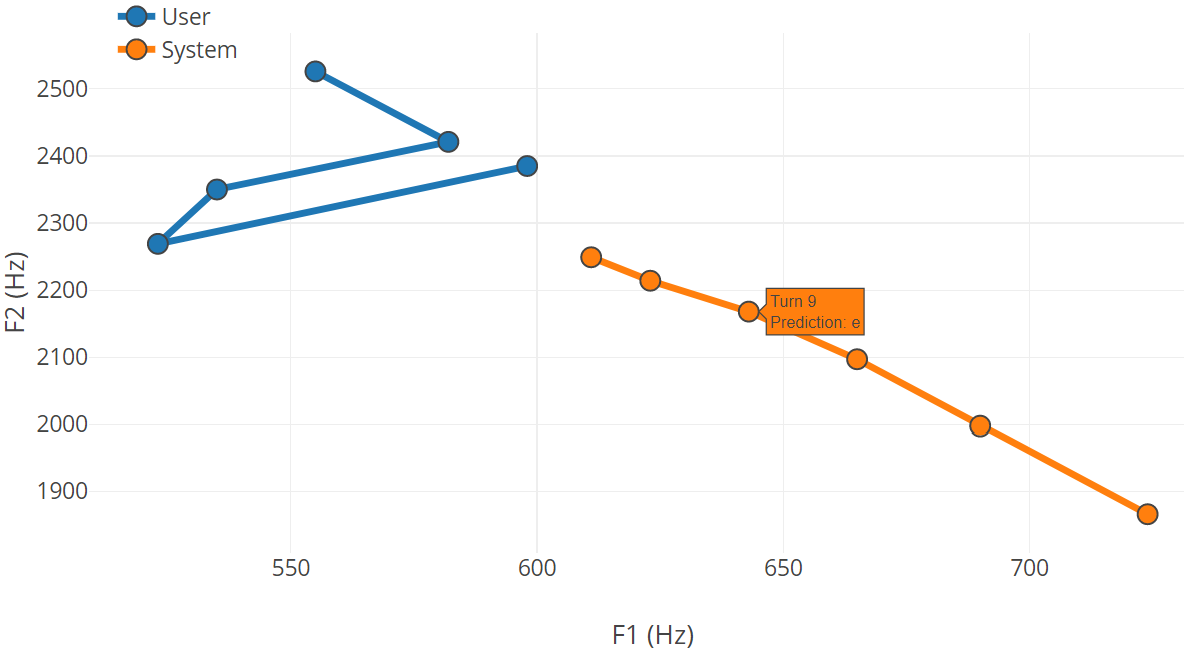
\includegraphics[width=\linewidth]{plot_area}
	\caption[Real-time dynamic visualization of phonetic changes]
		{The plot area showing the states of the feature \textipa{[E:]}~vs.~\textipa{[e:]} during an interaction.
		The system's (orange, bottom right) gradually adapts to the user's (blue, upper left) detected realizations.
		A prediction of the feature's current realization is given for both interlocutors.
		The text box shows the mouse-over annotation of the turn in which the system's realization changed its vowel category.}
	\label{fig:plot}
\end{figure}
%
Visualizations of the tracked features' changes over the course of the interaction are displayed in the upper right part of the screen.
Each feature is visualized separately, and new datapoints are dynamically added whenever applicable.
\Cref{fig:plot} shows an example of such a plot with several accumulated datapoints.
The type of a feature's plot can be defined based on its characteristics, e.g., bars for one-dimensional features and lined scatter plots for two-dimensional features.
These plots are generated using the Plotly library\footnote{\url{https://plot.ly}}, which provides some interactive functionalities.
Hovering over a datapoint in the plot reveals additional information, such as the turn in which it was added, or the realized variant of the feature produced in that turn, as predicted by its classifier (see \cref{subsec:classifiers_training}).

\subsubsection{Notification area}
\label{subsubsec:notification_area}

Whenever a message outside the content of the interaction needs to reach the user, it can be shown at the bottom right part of the screen.
Such messages may include indications of the system's activity, e.g., successful initialization of the interaction, warnings and errors while uploading files, etc.
The notifications can be colored blue, green, orange, or red to indicate the type of the message.

%\subsubsection{Settings and help}
%\label{subsubsec:settings_and_help}
%
%An additional modal window can be called, in which various settings can be changed, and some usage information is provided.
%Configurable settings include the convergence model parameters, domain file, \ac{gui} tweaks, and more.
%These settings can be modified at any point during the interaction, so that it is possible to experiment with different configurations in real-time.
%For persistent changes, it is also possible to edit the configuration file itself, which is loaded when the system starts.
%The usage tab explains the various functionalities of the system and how each area of the \ac{gui} works.
%It also lists special commands that can be executed from text field (used for simulating the user's input, as mentioned in \cref{subsubsec:interaction_area}).
%These commands include printing a short or detailed summary of the phonetic changes throughout the interaction, extracting the data from the features' plots (e.g., for further analysis), and more.
%\todo{screenshot with the settings tab}

\subsection{Customizations}
\label{subsec:models_and_cusomizations}

The system aims to offer a platform for \acp{sds} with convergence support that can be modified and customized according to the user's needs.
All of the aforementioned system components can be customized, at least to some extent.
This includes, among others, the phonetic convergence model, the features tracked by the system, and the dialogue domain.

\subsubsection{Tracked features}
\label{subsubsec:tracked_features}

The accommodation process is initiated by the phonetic features defined in the textual configuration file.
The process is triggered whenever a phoneme associated with a segmental phonetic feature is detected in a segment by the \ac{asr} or for a suprasegmental feature that potentially occurs for in segment.
The feature definitions may capture, for example, general tendencies or specific phonological rules, like schwa elision in German (see \cref{eq:schwa_elision_rule}).
As explained in \cref{subsec:computational_model}, each feature is detected and filtered based on its definition.
This definition can be easily changed to experiment with different accommodation effects.
An example for a feature definition is presented in \cref{subsec:setup_adjustments}.

\subsubsection{Dialogue domain}
\label{subsubsec:dialogue_domain}

The dialogue's flow is specified using OpenDial's XML-based format\footnote{\url{http://www.opendial-toolkit.net/user-manual/dialogue-domains}}.
This format offers a structure for building models, rules, and conditions, which define the \ac{dm} logic.
The rules connect between intents provided by the \ac{nlu} component to the output generated by the \ac{nlg} component.
Additional parameters are used to trigger processing for other modules of the \ac{sds}, like the \ac{asp} module in the system discussed here.
More details about building a domain file can be found in \citet{Lison2016opendial}.
The format of the domain file makes it easy to define new scenarios for the system, like different experimental settings.
Rules are written mostly using regular expressions, which makes it relatively easy also for non-technical users to modify the system's logic.
Since the \ac{dm} keeps track of parameters from all modules, the system's output can even be influenced by the state of the accommodation state in the \ac{asp} module.

\subsubsection{Speech processing}
\label{subsubsec:speech_processing}

Multiple components of the system deal with different aspects of speech processing.
As each module in the system can be replaced independently, different engines and models can be used.
For example, the \ac{asr} engine can be replaced for improving performance or adding support for additional languages.
The \ac{tts} component can be replaced as well, e.g., for changing the voice of the system or offering better control over phonetic manipulations.
The tool used for the phonetic analysis can be changed as well to improve accuracy or performance.
The models and tools described here are those that were used for the showcase presented in \cref{sec:showcase}.
The \ac{asr} component uses CMUSphinx\footnote{Sphinx4 version 5prealpha, \url{https://cmusphinx.github.io/}} \citep{Lamere2003sphinx}, with an extension to the phoneme emission functionality to provide the \ac{asp} module the phonetic input information it needs (see \cref{subsec:computational_model}).
The acoustic model and pronunciation dictionary were taken from CMUSphinx models\footnote{\url{https://sourceforge.net/projects/cmusphinx/files/Acoustic\%20and\%20Language\%20Models/German/}}.
A new language model was created especially for this purposes using SRILM \citep{Stolcke2002SRILM}.
All the segmental and suprasegmental analyses required for the measuring accommodation were done using Praat \citep{Boersma2018praat}.
MaryTTS \citep{LeMaguer2017uprooted, Schroeder2003mary} was used as the \ac{tts} engine of the system, with \texttt{bits1-hsmm} and \texttt{bits3-hsmm} for its female and male voices, respectively.

\section{Online and offline modes}
\label{sec:online_and_offline_modes}

\begin{figure}[t]
	\centering
	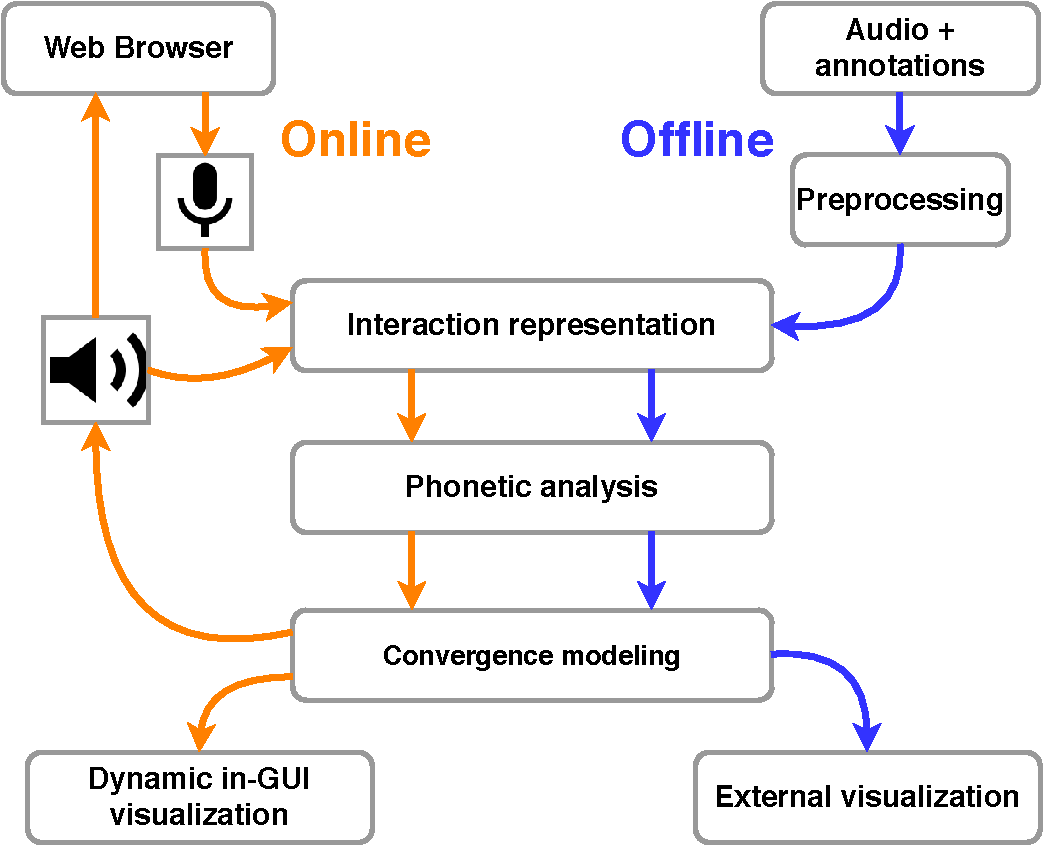
\includegraphics[width=0.85\linewidth]{online_offline_small}
	\caption[Online and offline modes of the responsive \acl{sds}]
		{Online (orange) and offline (blue) modes of the system.}
	\label{fig:online_offline_modes}
\end{figure}

The system can operate in two modes, as shown in \cref{fig:online_offline_modes}:
Online -- turn-based real-time interaction via the \ac{gui} (\cref{subsec:graphical_user_interface}); and offline -- on-demand analysis of existing interaction data, either from a recorded online session or a pre-recorded dataset.
The accommodation-related parts of the system (roughly corresponding to the \emph{server} and \emph{resources} blocks in \cref{fig:web-based_architecture}) are common to the two modes, which makes it easy to switch between the two.
The differences are in how the data is fed to the system and how the output is processed and visualized.
The main difference is that in the online mode the process is recurrent and both the user's input and the system's current state are acquired on the fly.
Depending on the scenario defined in the domain file, in online mode there could always be another turn, either of the user or the system, that will continue the interaction.
In the offline mode, the data scope is, by definition, finite.
Technically, the dataset is represented and processed the same way as online interactions, but there is no need to output the system's state to a user.
The common representation also makes it easy to compare pre-recorded interactions with live ones.
However, the output of the accommodation model after each turn is handled differently in both modes.
In online interactions, the output is sent on a turn-by-turn basis to both the web-based \ac{gui} for visualization (as in \cref{fig:plot}) and back to the user as auditory response from the system.
The offline mode doesn't need to interact with a user, so the entire analysis is saved together, along with some additional analyses that can only be preformed with complete interactions.
This output can then be used for further statistical analysis and be visualized separately using other tools (like those in \cref{fig:hds_dds_time,fig:synchrony_switchboard}).
For using the online mode, the system needs to run as a server and be accessed via a web browser.
The offline mode can be used either directly from the command line or programmatically from another application.
A mid-way usage is to manually load pre-recorded files via the \ac{gui} to simulate a live interaction, as explained in \cref{subsubsec:interaction_area}.
While this requires more time and manual effort, it lets the user observe the visualized gradual phonetic changes.

\section{Showcase: replicating a shadowing experiment}
\label{sec:showcase}

As a showcase of the system capabilities, it was utilized to replicate the shadowing experiment described in \cref{sec:convergence_to_natural_and_synthetic_stimuli}.
The experiment is designed to trigger phonetic convergence by confronting the participants with stimuli in which certain phonetic features are realized in a way different from their natural production.
This was done using the offline mode of the system, to simulate a real experiment and automate certain parts of it that would otherwise be performed manually.
The replication used the original stimuli and utterances of the participants.
However, analyses originally done post facto and to different extents manually, like detecting the realized variant, measuring the features' values, etc., are now done automatically.
This demonstrates an automated, reproducible execution, and also offers additional insights via classification of feature realizations and dynamic real-time visualizations.
Finally, using the system the experiment becomes more of a fluent dialogue rather than a experimental simulated interaction, which enhances its \ac{hci} nature.

\subsection{Setup}
\label{subsec:setup_adjustments}

For the experiment replication, two of the three segmental features investigated in the original experiment were used.
In addition to the \textipa{@}-length feature shown in \cref{subsec:computational_model} the feature \textipa{[E:]}~vs.~\textipa{[e:]} was included.
Both features are described in detail in \cref{subsubsec:target_features_HCIConv}, and \cref{tab:target_features} shows example stimulus sentences containing them.
As in the original experiment, the word containing the target features were embedded into 15 short carrier sentences and 25 filler sentences, in which none of the features occur (see \cref{app:shadow_experiment_stimul} for the full stimulus list).
Although both features' underlying values are gradual, they are perceived as two-way categorical variations.
To map these underlying values to a specific variant, a classifier was associated with each feature, as explained in \cref{subsec:classifiers_training}.
The definition of the \textipa{[E:]}~vs.~\textipa{[e:]} features was as follows:
%
%\begin{description}[labelindent=1.5cm, labelwidth=\widthof{\quad \bfseries calculation}]
%	\item[name]	ee\_E
%	\item[phoneme] EHH
%	\item[context] .* EHH .*
%	\item[initial] 451, 2116, 2763
%	\item[minimum] 300, 1500, 2500
%	\item[maximum] 750, 2900, 4800
%	\item[measure] formants
%	\item[calculation] decaying average
%	\item[sensitivity] 0.3
%\end{description}
%
\begin{Verbatim}[tabsize=4, commandchars=\\\{\}]
	- \textbf{`e\_E\_vowel'}:
			\textbf{phoneme}: EHH
			\textbf{context}: '.* EHH .*'
			\textbf{initial}: 450 2100
			\textbf{minimum}: 300 1500
			\textbf{maximum}: 750 2900
			\textbf{measure}: formants
			\textbf{calculation}: decaying average
			\textbf{sensitivity}: 0.3
\end{Verbatim}
%
%The value of the key \emph{measure} is \enquote{formants}, which means that this feature is evaluated by the segment's formant values (as specified in the corresponding signal processing script).
%The values of the \emph{minimum} and \emph{maximum} keys stand for the acceptable value range for this feature.
%This avoids distorted values due to \ac{asr} error and lets the user put their phonetic expertise to use.
\noindent
The values of the keys \texttt{minimum}, \texttt{maximum}, and \texttt{initial} stand for the first two formant frequencies.
The \texttt{calculation} method for this feature is \emph{decaying average} (\cref{eq:decaying_average}), which is similar to the regular average but with each value contributing exponentially less to the final value, so that the last (newest) exemplar contributes the most.
Adding such property to the measure gives more weight to new exemplars that were received chronologically closer to the current turn and thus makes the change more strongly influenced by the productions closer to the accommodation change.
Using this measure comes to support the analogy of the exemplar pool to short-term memory, which remembers recent events better than older ones.

Even though further aspects of the experiment could be automated, the experimental procedure stayed as faithful as possible to the procedure of the original experiment.
The domain file created for the showcase was designed to substitute the role of the experimenter in the shadowing phase (cf.\ \cref{fig:HCIConvFlow}), i.e., mainly presenting and playing the stimuli to the participant.
The stimulus order from the original experiment's baseline phase was preserved and semi-randomized in the shadowing phase using the same logic as in the original.
It was also configured to perform the transitions between the phases.
Although it should be assumed that the user indeed repeats the presented utterance, the system nonetheless verifies that the user's utterance matches the current stimulus using the customized language model described in \cref{subsubsec:speech_processing} before presenting the next stimulus.

% A shortened example of the shadowing phase's flow is shown in \cref{app:dialogue_example}.

%\begin{description}[labelindent=1.3cm, labelwidth=\widthof{\quad \textipa{[I\c{c}]}~vs.~\textipa{[Ik]}}]
%	\item [\textipa{[E:]}~vs.~\textipa{[e:]}] in word-medial $\langle$ä$\rangle$
%	\item [\textipa{[I\c{c}]}~vs.~\textipa{[Ik]}] in word-final $\langle$-ig$\rangle$
%	\item [\textipa{[\s{n}]}~vs.~\textipa{[@n]}] in word-final $\langle$-en$\rangle$
%\end{description}
%\noindent
%
\begin{table}[t]
	\centering
	\begin{tabularx}{\linewidth}{@{}*{5}{l}}
		\toprule
		
		War          	& das          			& Ger\textbf{\underline{ä}}t	& sehr          	& teuer? \\
		\emph{Was} 		& \emph{the} 			& \emph{device}           		& \emph{very} 		& \emph{expensive?} \\[0.3cm]
		
%		Ich          	& bin         			& sücht\textbf{\underline{ig}}	& nach				& Schokolade. \\
%		\emph{I}   		& \emph{am} 			& \emph{addicted}				& \emph{to} 		& \emph{chocolate.} \\[0.1cm]
		
		Wir         	& besuch\textbf{\underline{en}} 						& euch				& bald          & wieder. \\
		\emph{We} 		& \emph{will visit}		& \emph{you} 					& \emph{soon} 		& \emph{again.} \\
		\bottomrule
	\end{tabularx}
	\caption[Example sentence for selected phonetic features]
		{Examples of stimuli containing the target features.
		 Each sentence contains only one feature.
		 A list with all target and filler stimuli can be found in \cref{app:shadow_experiment_stimul} }
	\label{tab:target_features}
\end{table}

\subsection{Classifiers training}
\label{subsec:classifiers_training}

As mentioned above, a classifier can be defined for each tracked feature to let the system determine to which realization category each encountered belongs.
This automates the annotation otherwise done manually by the experimenter during or after the experiment.
In the original shadowing experiment, this includes both the determination of the participants' preferred variation in the baseline phase and the annotation of the participants' realizations in the shadowing phase.
To that end, the associated classifier provides real-time classifications for both the user's and the system's realizations of that feature.
This not only saves time, but also helps to prevent inconsistencies that on-the-fly manual annotation might yield.
With this information available, more meaningful insights can be gained into the variation dynamics over the course of the interaction.
In other applications, like \acp{capt}, this information may be taken into account when deciding on the system's next turn.
The classifiers for the replicated experiment were trained on datasets corresponding to the target features' ranges.
The \textipa{@}-length classifier trained to classify segments shorter and longer than \SI{30}{\milli\second}, and the \textipa{e:/E:} classifier was trained on F1 and F2 values of these vowels produced by female speakers (since for the replication a female participant was chosen as well as a female voice for the system).
While training prior to the interactions is generally sufficient, online fine-tuning is also possible to update a feature's classifier whenever requested by the user, e.g., every time the accommodation model is updated.

Here, a \ac{smo} \citep{Platt1999fast, Platt1998sequential} implementation of the \ac{svm} classifier \citep{Vapnik1998support, Joachims2005support} was used, as the two-way categories of these features are expected to be linearly separable.
Each turn's predictions dynamically added as interactive annotations to the visualization of the relevant features, as illustrated in \cref{fig:plot}.
The training data used for each classifier contains only the productions of the corresponding target feature from a single stimulus set, since these are the productions to which the participants were exposed during the experiment.
This provides relatively few -- but at the same time very precise -- datapoints for each classifier,
which were obtained using the same signal processing technique as the data collected in the experiment.
As explained in \cref{subsubsec:stimuli_participant_hci}, multiple stimulus sets were used in the experiment.
The classification of the system's production was performed based on the stimulus type the participant listened to.
For instance, a classifier trained on the natural stimuli was used when the participant was listening to this stimulus set.

\subsection{Validation}
\label{subsec:validation}

\begin{table}[t]
	\centering
	\begin{tabularx}{\linewidth}{X*{4}{S[table-format=2.1]}}
		\toprule
		sensitivity (\numrange{0}{1}) &  0.2 &  0.3 &  0.4 &  0.5 \\
		adoption (\si{\percent})      & 79   & 86   & 75   & 69   \\
		\bottomrule
	\end{tabularx}
	\caption{The system's convergence degree with different degrees of sensitivity.}
	\label{tab:validation_baseline}
\end{table}

%The validation for the feature \textipa{[E:]}~vs.~\textipa{[e:]} is shown here as a representative example for the phonetic adaptation capability of the system.
For the baseline phase, the degree to which the underlying convergence model accumulated enough data to adopt the user's variant of the feature was examined.
Higher adoption rate indicates a more stable preferred variant of the participant.
The participant's preferred variants was determined based on the majority vote at the end of this phase, as in the original experiment.
For example, if the user realized one variant twice and another three times, the latter was considered the preferred one.
\Cref{tab:validation_baseline} shows the adoption rates of the user's preferred variant as percentages of the mean preferred variant using different values of the \emph{convergence rate} parameter (see \cref{sec:parameters}).
Interestingly, higher values do not necessarily result in higher percentages, due to systematic over-shooting the participant's production in each utterance.
The value 0.3 provided the highest results and was therefore used through the rest of the replication.
See \cref{fig:validation_sensitivity} for visualized examples of the convergence rate's influence.
%
\begin{figure}[t]
	\centering
	\subfigure[The effect of different convergence rates on the change of
			   the system's representation toward the participant's \emph{mean value} for the two-dimensional feature \textipa{[e:]} vs.\ \textipa{[E:]} using decaying average ($\mu = 0.3$).
			   The points represent the calculation steps of the rates 0.1 (red circles), 0.5 (yellow tiranlges), and 0.9 (green rectangles).
			   Each point is the new value calculated after encountering a new exemplar.
			   The common starting point at the top left is the feature's defined initial value.
			   The ellipses represent confidence levels of \SI{90}{\percent}, \SI{50}{\percent}, and \SI{10}{\percent}.]
		{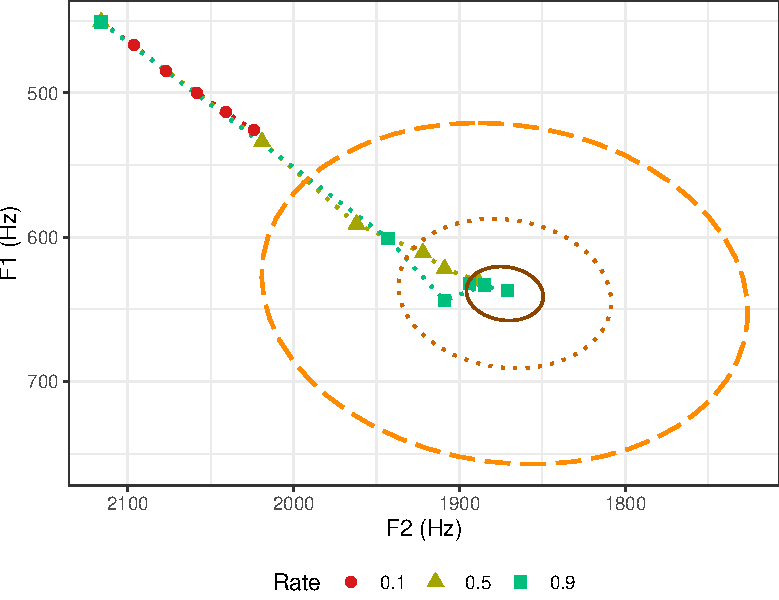
\includegraphics[width=0.47\textwidth]{ee_E_decaying_0.3}
	\label{fig:e_E_bullseye}}
	\hfill
	\subfigure[The effect of different convergence rates for the one-dimensional feature \textipa{@}-length.
			   The bars' height represent the feature's values on the y-axis with the calculation method set to simple average.
			   The x-axis enumerates the feature's updates.
			   The \emph{exemplar} bar shows the feature’s last added exemplar, and the \emph{average} bar
			   is the value of the feature after adding the last exemplar to the pool.
			   Note that the 0-th update appears empty since the initial value of the feature was set to 0.]
		{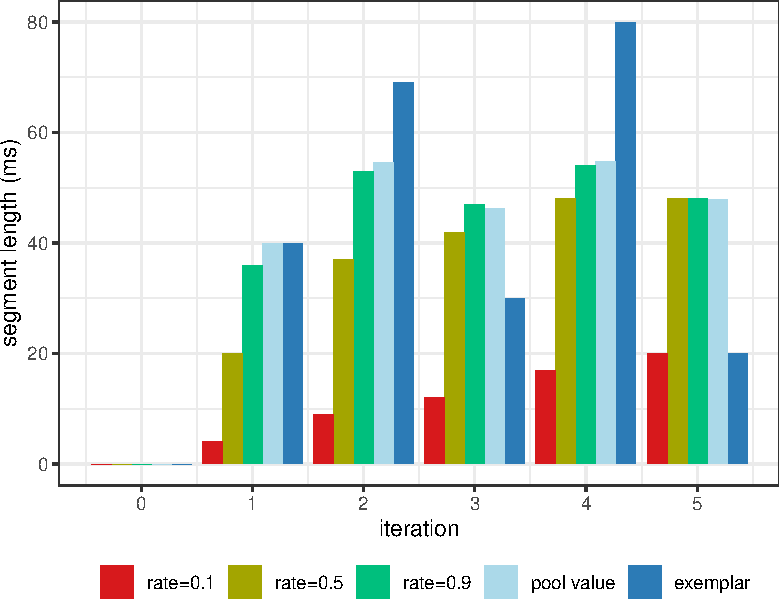
\includegraphics[width=0.47\textwidth]{schwa_comp_010509}
	\label{fig:schwa_length_bars}}
	\caption[Influence of difference convergence rates on the system's accommodation]
		{Illustration of the effect of different convergence rates on the updates of the system's realization of a two-dimensional feature (left) and a one-dimensional feature (right).}
	\label{fig:validation_sensitivity}
\end{figure}
%
After obtaining the preference of each participant, the degree of convergence was examined per utterance in the shadowing phase.
The participants were grouped based on their convergence behavior in the original experiment:
One group of participants showed low to no tendency to converge (converged in $\le$\SI{10}{\percent} of their utterances),
the second had varying degrees of convergence (\SIrange{10}{90}{\percent}),
and the third group of participants who were very sensitive to the stimuli ($\ge$\SI{90}{\percent}).
This grouping enables analyses based on collective vocal behaviors instead of individual differences.
The groups were labeled \emph{Low} (\SI{23}{\percent} of participants), \emph{Mid} (\SI{50}{\percent}), and \emph{High} (\SI{27}{\percent}), respectively.
For validation purposes, the shadowing phase was treated as an annotation task of the realized variation in the participants' utterances, where a correct annotation (system produces same variation as the participant) indicates convergence.
The three \enquote{annotators} are the stimuli themselves (\emph{Stim}), the online classification of the system's representation of the feature (\emph{Sys}), and labels from the training dataset used as references (\emph{Ref}).
The Cohen's kappa ($\kappa$) values\footnote{Calculated by the \texttt{kappa2} command of the \texttt{irr} R package, \url{https://cran.r-project.org/package=irr}} are shown in \cref{tab:showcase_results}.
%As expected, the \emph{Low} group has the lowest scores, since these are the participants that converged the least as a whole.
%As \cref{tab:showcase_results} shows, convergence was found in \SI{48}{\percent} of the utterances for \emph{Sys-Stim} and \emph{Ref-Stim} but only in \SI{66}{\percent} for \emph{Ref-Sys}, which means that convergence was found in different instances.
%\todo{not clear what the sentence above wants to say}
\cref{tab:showcase_results} shows that \emph{Ref-Sys} has $\kappa = 0.27$ (fair agreement) for the \emph{Mid} group, but lower scores for the two other groups.
This indicates that the reference values, which supposedly represent some universal average of the feature, indeed match the production of the participants that didn't deviate too greatly from their base production values, which reinforces the fact that the stimuli's influence on them was limited to either direction.
The $\kappa$ values for \emph{Sys-Stim} describe how the system's representations matched the stimuli presented to the participants.
Since the system accommodates to the participants' performance, these values exhibit how similarly the system's productions were to the productions of each participant group.
The \emph{High} group has $\kappa = 0.81$ (strong agreement), indicating a high similarity between these participants and the system, as expected.
Contrarily, the $\kappa$ value for the \emph{Low} group is -0.57 (moderate negative agreement), showing that no convergence -- and potentially even divergence -- occurred with these participants.
% kappa itepratation classes taken from http://www.statisticshowto.com/cohens-kappa-statistic/
These results show that the online predictions made by the system presented here are capable of providing additional insights regarding the accommodation degrees occurring in an interaction.
%
\begin{table}[t]
	\centering
	\caption[Cohen's Kappa scores of system's validation]
		{Percentage of convergence cases and $\kappa$ scores of the three-way convergence comparison for the three participant groups.
		Positive $\kappa$ scores mean agreement between the annotations (here, the feature's realization category) and negative scores indicate disagreement.
		Scores close to zero point to an agreement occurring by chance.}
	\label{tab:showcase_results}
	\begin{tabularx}{\linewidth}{X
								 *{3}{S[table-format=2.0]}
								 @{\hskip 1.4cm}
								 *{3}{S[table-format=1.2, table-space-text-pre={$-$}, table-space-text-post={\,***}]}}
		\toprule
		\multirow{2}{*}{Group} &
		\multicolumn{3}{c}{Convergence cases (\si{\percent})} &
		\multicolumn{3}{c}{Cohen's Kappa ($\kappa$)}\\[0.2cm]
		&
		{\emph{Sys}-\emph{Stim}} & {\emph{Ref}-\emph{Stim}} & {\emph{Ref}-\emph{Sys}} &
		{\emph{Sys}-\emph{Stim}} & {\emph{Ref}-\emph{Stim}} & {\emph{Ref}-\emph{Sys}}\\
		\midrule
		Low		& {<1} &  7 & 16 & -0.57\,*** & -0.08		& 0.17		\\
		Mid		&  22  & 23 & 32 & -0.15\,*   & -0.15\,*	& 0.27\,***	\\
		High	&  26  & 18 & 18 &  0.81\,*** & -0.04		& 0.03		\\[0.2cm]
		All		&  48  & 48 & 66 & -0.11\,*   & -0.13\,**	& 0.21\,***	\\
		\bottomrule
	\end{tabularx}
	\flushleft{\footnotesize \emph{* $p < 0.05$, ** $p < 0.01$, *** $p < 0.001$}}
\end{table}